\documentclass[11pt]{article}

\usepackage[letterpaper,left=85.5pt,right=87pt,top=70.5pt,bottom=78.8pt,headheight=0pt,headsep=0pt]{geometry}
\usepackage[spanish,es-noshorthands]{babel}
\usepackage{fontspec}
\usepackage{xcolor}
\usepackage{graphicx}
\usepackage{enumitem}
\usepackage{array}
\usepackage{tabularx}
\usepackage{longtable}
\usepackage{booktabs}
\usepackage{colortbl}
\usepackage{caption}
\usepackage{fancyhdr}
\usepackage{ragged2e}
\usepackage{microtype}
\usepackage[hidelinks]{hyperref}

\definecolor{claudia}{HTML}{1F6FEB}
\definecolor{claudiadark}{HTML}{17324D}
\definecolor{tablehead}{HTML}{E7E6E6}

\setsansfont{Arial}
\renewcommand{\familydefault}{\sfdefault}
\setlength{\parindent}{0pt}
\setlength{\parskip}{8pt}
\linespread{1.0}
\setlength{\emergencystretch}{2em}
\setlist[itemize]{leftmargin=1.25em,itemsep=0.10em,topsep=0.18em,parsep=0pt}
\setlist[enumerate]{leftmargin=1.45em,itemsep=0.10em,topsep=0.18em,parsep=0pt}

\pagestyle{fancy}
\fancyhf{}
\fancyfoot[R]{\fontsize{12}{14.6}\selectfont\thepage}
\renewcommand{\headrulewidth}{0pt}
\renewcommand{\footrulewidth}{0pt}

\captionsetup{font=small,labelfont=bf,labelsep=colon,justification=centering,skip=3pt}
\makeatletter
\newcommand{\ManualHeading}[1]{%
  \clearpage
  \phantomsection
  \label{#1}%
  \begin{center}\normalfont\fontsize{11}{14.6}\selectfont\bfseries\csname heading@#1\endcsname\end{center}%
  \vspace{4pt}%
}
\newcommand{\HeadingText}[2]{\expandafter\def\csname heading@#1\endcsname{#2}}
\makeatother

\newcommand{\Subheading}[1]{\par\vspace{5pt}{\normalfont\fontsize{11}{14.6}\selectfont\bfseries #1}\par\vspace{3pt}}
\newcommand{\TOCMain}[2]{\noindent\makebox[0.88\linewidth][l]{\strut\textbf{#1}\dotfill}\makebox[0.10\linewidth][r]{\strut\pageref{#2}}\par}
\newcommand{\TOCSub}[2]{\noindent\makebox[0.045\linewidth][l]{\strut}\makebox[0.845\linewidth][l]{\strut #1\dotfill}\makebox[0.10\linewidth][r]{\strut\pageref{#2}}\par}

\newcommand{\ManualSection}[2]{%
  \expandafter\def\csname heading@#1\endcsname{#2}%
  \ManualHeading{#1}%
}

\newcommand{\ShotSingle}[3][0.92\textwidth]{%
  \begin{center}
    \includegraphics[width=#1,height=3.65in,keepaspectratio]{#2}
    \FigureCaption{#3}
  \end{center}
}
\newcommand{\FigureCaption}[1]{%
  \par\vspace{1pt}%
  \refstepcounter{figure}%
  \begin{center}\fontsize{11}{14.6}\selectfont #1\end{center}%
  \vspace{2pt}%
}
\newcommand{\ShotPair}[4][0.47\textwidth]{%
  \begin{center}
    \begin{minipage}[t]{0.49\linewidth}\centering
      \includegraphics[width=#1,height=3.25in,keepaspectratio]{#2}
    \end{minipage}\hfill
    \begin{minipage}[t]{0.49\linewidth}\centering
      \includegraphics[width=#1,height=3.25in,keepaspectratio]{#3}
    \end{minipage}
    \FigureCaption{#4}
  \end{center}
}

\begin{document}
\pagenumbering{gobble}
\fontsize{11}{14.6}\selectfont

\begin{center}
  \vspace*{-0.34in}
  {Manual de Usuario de\par}
  \vspace{0pt}
  {ClaudIA\par}
  \vspace{0.07in}
  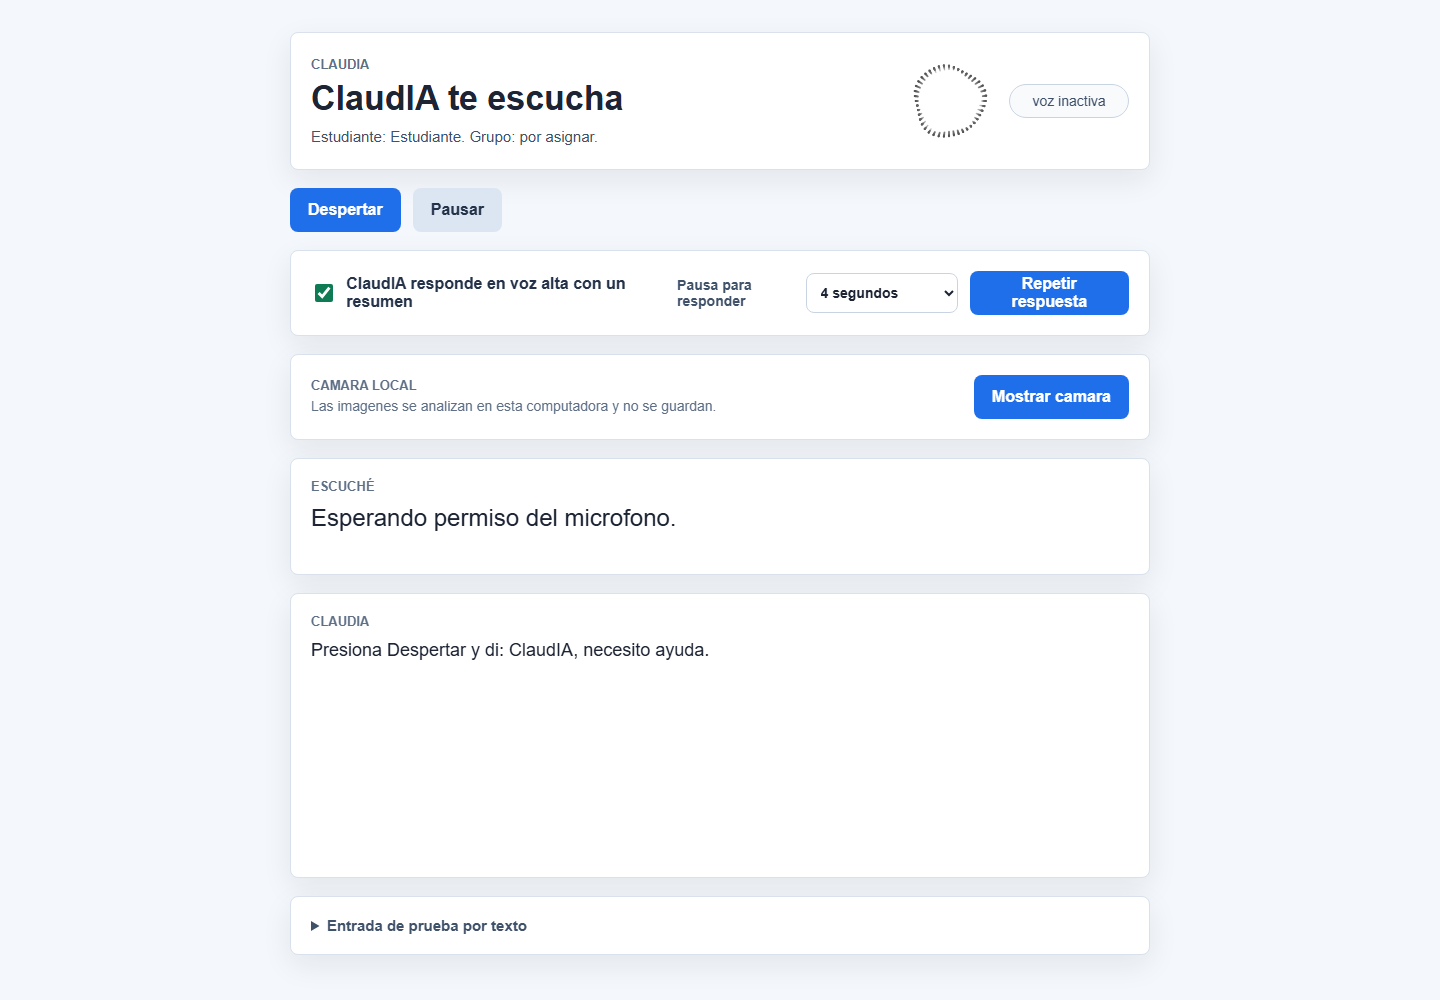
\includegraphics[width=5.12in,height=3.49in,keepaspectratio]{assets/interfaz_inicial.png}
\end{center}

\vspace{-0.17in}
\begin{tabularx}{\textwidth}{@{}>{\bfseries}p{1.45in}X@{}}
\toprule
Proyecto & ClaudIA: Sistema Inteligente de Acompañamiento Didáctico para Grupos DGETI \\
Código & 26-AT625 \\
Manual & Versión 1.0 \\
Plantel & CETis 20, Ciudad del Carmen, Campeche \\
Subsistema & DGETI-SEMS-SEP \\
\bottomrule
\end{tabularx}

\clearpage
\pagenumbering{arabic}
\setcounter{page}{1}

\makeatletter
\HeadingText{indice}{Índice}
\makeatother
\ManualHeading{indice}
{\fontsize{11}{15.7}\selectfont
\TOCMain{Introducción}{intro}
\TOCMain{Aviso de privacidad}{privacidad}
\TOCMain{Requisitos previos}{requisitos}
\TOCMain{Requisitos de usuario y acceso}{acceso}
\TOCMain{Puesta en marcha}{instalacion}
\TOCMain{Interfaz inicial}{interfaz}
\TOCMain{Activación por voz}{voz}
\TOCMain{Controles de escucha}{controles}
\TOCMain{Entrada por texto}{texto}
\TOCMain{Identificación del estudiante y grupo}{contexto}
\TOCMain{Comandos básicos}{comandos}
\TOCMain{Verificación del sistema}{verificacion}
\TOCMain{Inicio de la tutoría}{iniciar}
\TOCMain{Secuencia de acompañamiento}{secuencia}
\TOCMain{Explicación guiada}{explicacion}
\TOCMain{Práctica y retroalimentación}{practica}
\TOCMain{Recorrido diario del estudiante}{recorrido}
\TOCMain{Modo docente}{docente}
\TOCMain{Preparación de una clase}{clase}
}
\clearpage

{\fontsize{11}{15.7}\selectfont
\TOCMain{Panel y resumen docente}{panel}
\TOCMain{Cámara y detección de presencia}{camara}
\TOCMain{Controles de privacidad}{privacidad_camara}
\TOCMain{Materiales y documentos}{documentos}
\TOCMain{Presentaciones}{presentaciones}
\TOCMain{Problemas de inicio}{problemas_inicio}
\TOCMain{Problemas de voz}{problemas_voz}
\TOCMain{Problemas de cámara}{problemas_camara}
\TOCMain{Problemas del tutor y la IA}{problemas_ia}
\TOCMain{Problemas de presentaciones}{problemas_presentaciones}
\TOCMain{Mantenimiento del usuario}{mantenimiento_usuario}
\TOCMain{Mantenimiento técnico}{mantenimiento_admin}
\TOCMain{Actualización y respaldo}{respaldo}
\TOCMain{Glosario A-F}{glosario_a}
\TOCMain{Glosario G-Z}{glosario_b}
\TOCMain{Apéndices}{apendices}
\TOCMain{Limitaciones, soporte y control}{cierre}
}

\HeadingText{intro}{Introducción}
\ManualHeading{intro}
Este manual explica cómo preparar y operar ClaudIA como estación de acompañamiento didáctico en el aula. Está dirigido a estudiantes, docentes y responsables técnicos del plantel.

El usuario formula una consulta oral, recibe una respuesta hablada y avanza con preguntas, ejemplos o pistas. Cuando el audio no es confiable, puede recurrir al texto. El docente mantiene la conducción pedagógica y recibe información agregada.

\Subheading{Qué encontrará en este manual}
\begin{itemize}
  \item Preparación del equipo y verificación de los componentes.
  \item Activación de la voz, la entrada de texto y la cámara.
  \item Registro del estudiante y del grupo activo.
  \item Uso del tutor, la práctica y la retroalimentación.
  \item Herramientas para el docente, documentos y presentaciones.
  \item Solución de problemas, mantenimiento y recomendaciones.
\end{itemize}

\Subheading{Alcance}
ClaudIA es una herramienta complementaria y su alcance se limita al apoyo didáctico. Quedan fuera los diagnósticos de salud, las calificaciones automáticas y la lectura de cuadernos para resolver ejercicios.

\HeadingText{privacidad}{Aviso de privacidad}
\ManualHeading{privacidad}
La voz es el medio principal de interacción. La cámara aporta una señal local de presencia o contexto general. El sistema conserva únicamente la información necesaria para sostener la sesión y registrar el progreso autorizado.

\Subheading{Finalidad}
\begin{itemize}
  \item Ofrecer explicaciones y práctica guiada.
  \item Mantener el contexto del estudiante y del grupo.
  \item Generar resúmenes pedagógicos para el docente.
\end{itemize}

\Subheading{Controles aplicados}
\begin{itemize}
  \item La cámara no identifica rostros ni infiere emociones.
  \item El video no se guarda por defecto.
  \item El micrófono y la cámara pueden pausarse o desactivarse.
  \item Las claves de IA permanecen fuera de la conversación y del código público.
  \item El contexto temporal puede borrarse al finalizar una sesión.
\end{itemize}

\Subheading{Derechos ARCO}
El estudiante o su tutor puede solicitar acceso, rectificación, cancelación u oposición al tratamiento de sus datos mediante el canal institucional que determine el plantel.

\HeadingText{requisitos}{Requisitos previos}
\ManualHeading{requisitos}
Antes de utilizar la estación, verifique que el equipo cumpla las condiciones mínimas de operación.

\Subheading{Requisitos técnicos}
\begin{itemize}
  \item Computadora con Windows, macOS o Linux.
  \item Node.js 20 o superior.
  \item Chrome o Edge actualizado.
  \item Micrófono y bocina conectados.
  \item Python 3 con OpenCV únicamente si se usará la cámara.
\end{itemize}

\Subheading{Conectividad}
ClaudIA puede iniciar sin conexión para consultar comandos locales. Las respuestas generativas requieren conexión y un proveedor de IA configurado. La estación debe tolerar interrupciones sin perder el estado general de la sesión.

\Subheading{Conocimientos mínimos del usuario}
No se requieren conocimientos técnicos. El usuario debe saber hablar de forma clara, leer las instrucciones de pantalla y detener la sesión cuando sea necesario.

\HeadingText{acceso}{Requisitos de usuario y acceso}
\ManualHeading{acceso}
Cada sesión comienza con una identificación mínima del contexto escolar. No se requiere una cuenta en línea.

\Subheading{Información necesaria}
\begin{itemize}
  \item Nombre o identificador del estudiante.
  \item Grupo activo.
  \item Tema o actividad que se desea trabajar.
  \item Rol de uso: estudiante, docente o administrador.
\end{itemize}

\Subheading{Recomendaciones}
\begin{itemize}
  \item No proporcione datos personales innecesarios.
  \item Utilice un identificador breve cuando el grupo sea amplio.
  \item Verifique el contexto antes de iniciar una lección.
  \item Al finalizar, use el cierre de sesión para preparar la estación para otra persona.
\end{itemize}

\HeadingText{instalacion}{Puesta en marcha}
\ManualHeading{instalacion}
La instalación puede realizarla el responsable técnico del plantel. El estudiante sólo necesita encontrar la estación preparada y activa.

\Subheading{Preparación local}
\begin{enumerate}
  \item Abra una terminal en la carpeta del proyecto.
  \item Ejecute \texttt{npm install}.
  \item Ejecute \texttt{npm run setup}.
  \item Ejecute \texttt{npm run doctor}.
  \item Inicie la interfaz con \texttt{npm start}.
  \item Abra \texttt{http://127.0.0.1:3000}.
\end{enumerate}

\Subheading{Clave del proveedor}
El responsable debe colocar la clave de IA en el archivo local \texttt{.env}. La clave no se comparte por voz, no se muestra en pantalla y no debe incorporarse al repositorio.

\Subheading{Comprobación rápida}
El diagnóstico debe confirmar Node.js, configuración local, proveedor de IA y servicio web. Si algún elemento falta, consulte la sección de solución de problemas antes de iniciar una clase.

\HeadingText{interfaz}{Interfaz inicial}
\ManualHeading{interfaz}
La pantalla principal organiza el estado de la sesión, los controles y los paneles de transcripción y respuesta.

\begin{enumerate}
  \item \textbf{Estado y contexto:} identifican al estudiante, el grupo y la disponibilidad de la voz.
  \item \textbf{Controles de voz:} permiten iniciar, pausar o repetir una intervención.
  \item \textbf{Cámara local:} activa la vista de presencia cuando la actividad lo requiere.
  \item \textbf{Transcripción y respuesta:} muestran lo que entendió la estación y la orientación que ofrece.
  \item \textbf{Entrada por texto:} permite continuar cuando el micrófono no está disponible.
\end{enumerate}

\ShotSingle[0.82\textwidth]{assets/interfaz_inicial.png}{Figura 1: Interfaz principal de ClaudIA.}

\HeadingText{voz}{Activación por voz}
\ManualHeading{voz}
La voz es el canal principal. El estudiante habla con la estación sin instalar una aplicación adicional.

\Subheading{Primera activación}
\begin{enumerate}
  \item Pulse \textbf{Despertar}.
  \item Conceda permiso al micrófono si el navegador lo solicita.
  \item Espere a que el indicador muestre que la estación escucha.
  \item Hable con una frase breve, por ejemplo: «ClaudIA, necesito ayuda».
\end{enumerate}

La estación convierte la voz en texto, confirma lo que entendió y procesa la intención. Si la transcripción no es confiable, solicita repetir antes de responder.

\Subheading{Buenas prácticas}
\begin{itemize}
  \item Hable a una distancia estable del micrófono.
  \item Evite que varias personas hablen al mismo tiempo.
  \item Formule una pregunta por intervención.
  \item Use frases como «dame una pista» o «no entendí».
\end{itemize}

\HeadingText{controles}{Controles de escucha}
\ManualHeading{controles}
La estación permite controlar cuándo escucha y cuánto tiempo espera antes de procesar una intervención.

\Subheading{Pausa para responder}
El selector ofrece esperas de 2.5, 4 o 6 segundos. Una pausa breve agiliza la interacción; una pausa mayor ayuda cuando el estudiante explica un razonamiento largo.

\Subheading{Pausar y reanudar}
\begin{itemize}
  \item Pulse \textbf{Pausar} para suspender temporalmente la escucha.
  \item Confirme que el estado indique que ClaudIA no está escuchando.
  \item Pulse \textbf{Despertar} para continuar.
  \item Cierre la sesión al cambiar de estudiante.
\end{itemize}

\Subheading{Repetir respuesta}
El botón \textbf{Repetir respuesta} vuelve a leer la respuesta más reciente sin repetir la consulta académica.

\HeadingText{texto}{Entrada por texto}
\ManualHeading{texto}
La entrada escrita permite probar la estación y continuar cuando el micrófono falla o el ruido del aula interfiere.

\begin{enumerate}
  \item Abra el panel \textbf{Entrada de prueba por texto}.
  \item Escriba una instrucción o pregunta.
  \item Pulse \textbf{Enviar}.
  \item Espere la respuesta en el panel de ClaudIA.
\end{enumerate}

\Subheading{Ejemplos}
\begin{itemize}
  \item \texttt{ayuda}
  \item \texttt{mostrar lecciones}
  \item \texttt{iniciar lección fracciones básicas}
  \item \texttt{explicame fracciones}
  \item \texttt{estado de visión}
\end{itemize}

La escritura funciona como alternativa de acceso; la conversación oral sigue siendo la experiencia principal.

\HeadingText{contexto}{Identificación del estudiante y grupo}
\ManualHeading{contexto}
El contexto escolar separa la conversación, el progreso y la memoria de cada estudiante.

\Subheading{Registrar estudiante}
Escriba o pronuncie:
\begin{center}\texttt{usar estudiante Estudiante de prueba}\end{center}

\Subheading{Registrar grupo}
Después del estudiante, indique el grupo:
\begin{center}\texttt{usar grupo 5A}\end{center}

\ShotPair[0.47\textwidth]{assets/contexto_estudiante.png}{assets/contexto_grupo.png}{Figuras 2 y 3: Registro del estudiante y del grupo activo.}

Cuando cambia la identidad o el grupo, la conversación temporal se reinicia para evitar mezclar contextos.

\HeadingText{comandos}{Comandos básicos}
\ManualHeading{comandos}
ClaudIA reconoce lenguaje natural y comandos breves. La palabra \texttt{ayuda} muestra la lista completa.

\begin{center}
\begin{tabularx}{\textwidth}{@{}>{\ttfamily}p{2.05in}>{\raggedright\arraybackslash}X@{}}
\toprule
\normalfont\textbf{Comando} & \textbf{Acción} \\
\midrule
ayuda & Muestra los comandos disponibles \\
usar estudiante & Identifica al estudiante activo \\
usar grupo & Identifica el grupo activo \\
mostrar sesión & Presenta el estado de la sesión \\
reiniciar sesión & Limpia el contexto temporal \\
mostrar lecciones & Lista los temas disponibles \\
iniciar lección & Abre una lección concreta \\
empezar clase & Inicia el acompañamiento del tutor \\
explicame & Solicita una explicación guiada \\
hacer ejercicio & Genera una práctica breve \\
mi respuesta es & Envía una respuesta para revisión \\
activar voz & Habilita el canal de voz \\
estado de visión & Revisa Python, OpenCV y cámara \\
\bottomrule
\end{tabularx}
\end{center}

\ShotSingle[0.72\textwidth]{assets/comandos_ayuda.png}{Figura 4: Respuesta del comando de ayuda.}

\HeadingText{verificacion}{Verificación del sistema}
\ManualHeading{verificacion}
Antes de usar la estación con estudiantes, ejecute esta prueba de aceptación.

\begin{enumerate}
  \item Confirme que la interfaz abre en el navegador.
  \item Verifique que los botones de voz estén disponibles.
  \item Escriba \texttt{ayuda} y compruebe la respuesta.
  \item Registre un estudiante y un grupo de prueba.
  \item Ejecute \texttt{mostrar lecciones}.
  \item Inicie una explicación y escuche la respuesta.
  \item Revise el estado de la cámara si se utilizará en la actividad.
\end{enumerate}

\ShotSingle[0.76\textwidth]{assets/mostrar_lecciones.png}{Figura 5: Verificación mediante el listado de lecciones.}

Si todas las pruebas responden correctamente, la estación puede pasar a uso supervisado.

\HeadingText{iniciar}{Inicio de la tutoría}
\ManualHeading{iniciar}
El modo tutor comienza cuando el estudiante solicita apoyo. ClaudIA se presenta, pregunta por el tema y pide identificar la parte que no se comprende.

\begin{enumerate}
  \item Registre al estudiante y el grupo.
  \item Diga o escriba \texttt{empezar clase}.
  \item Escuche la respuesta inicial.
  \item Indique el tema, por ejemplo: \texttt{explicame fracciones}.
\end{enumerate}

\ShotSingle[0.76\textwidth]{assets/iniciar_tutor.png}{Figura 6: Inicio del acompañamiento del tutor.}

La estación no comienza resolviendo el ejercicio. Primero identifica el objetivo y el punto donde el estudiante necesita apoyo.

\HeadingText{secuencia}{Secuencia de acompañamiento}
\ManualHeading{secuencia}
Cada interacción sigue una progresión pedagógica:
\begin{enumerate}
  \item \textbf{Objetivo:} confirmar qué se desea aprender.
  \item \textbf{Intento:} solicitar una explicación o solución inicial.
  \item \textbf{Pista:} ofrecer una regla o pregunta guía.
  \item \textbf{Nuevo intento:} permitir que el estudiante corrija.
  \item \textbf{Comprobación:} pedir una justificación.
  \item \textbf{Derivación:} consultar al docente cuando el bloqueo persiste.
\end{enumerate}

\Subheading{Qué evitar}
\begin{itemize}
  \item Solicitar únicamente «la respuesta».
  \item Copiar una explicación sin intentar comprenderla.
  \item Hablar antes de que ClaudIA termine de responder.
  \item Mantener la cámara activa sin una actividad relacionada.
\end{itemize}

\HeadingText{explicacion}{Explicación guiada}
\ManualHeading{explicacion}
Una solicitud clara produce una respuesta más útil.

\Subheading{Formas recomendadas}
\begin{itemize}
  \item «Explícame fracciones con un ejemplo cotidiano».
  \item «No entiendo por qué cambié de signo».
  \item «Dame una pista para resolver esta ecuación».
  \item «Compara mi respuesta con el procedimiento».
\end{itemize}

\ShotSingle[0.76\textwidth]{assets/explicacion_fracciones.png}{Figura 7: Explicación guiada de fracciones.}

El estudiante debe responder con sus palabras. Si no puede, puede pedir una pregunta más sencilla o un ejemplo distinto.

\HeadingText{practica}{Práctica y retroalimentación}
\ManualHeading{practica}
Después de una explicación, ClaudIA puede proponer práctica breve.

\begin{enumerate}
  \item Solicite \texttt{hacer ejercicio}.
  \item Lees el problema y resuélvelo.
  \item Envía la respuesta con \texttt{mi respuesta es} seguida del resultado.
  \item Revisa la retroalimentación y explica el procedimiento.
  \item Repite con otro caso si la respuesta necesita ajustes.
\end{enumerate}

Los ejercicios avanzan por dificultad. ClaudIA pregunta antes de mostrar el procedimiento completo, revisa el razonamiento y ofrece un resumen oral del avance.

\HeadingText{recorrido}{Recorrido diario del estudiante}
\ManualHeading{recorrido}
\begin{enumerate}
  \item Confirme que su nombre y grupo aparecen en pantalla.
  \item Pulse \textbf{Despertar} o abra la entrada de texto.
  \item Indique el tema o la duda.
  \item Escuche la confirmación de ClaudIA.
  \item Responda a la pregunta de seguimiento.
  \item Solicite una pista cuando la necesite.
  \item Intente nuevamente y explique el resultado.
  \item Al terminar, solicite un resumen y deje la estación lista para la siguiente persona.
\end{enumerate}

El panel \textbf{Escuché} conserva la transcripción y el panel \textbf{ClaudIA} muestra la respuesta completa.

\HeadingText{docente}{Modo docente}
\ManualHeading{docente}
El docente puede utilizar la misma estación para organizar una clase y obtener recursos de apoyo.

\Subheading{Ventajas}
\begin{itemize}
  \item Recupera el tema de la clase anterior.
  \item Mantiene el grupo activo.
  \item Propone preguntas iniciales.
  \item Genera material visual para el tema actual.
\end{itemize}

\Subheading{Recomendación}
Revise los temas, las preguntas y las presentaciones antes de utilizarlos frente al grupo.

\HeadingText{clase}{Preparación de una clase}
\ManualHeading{clase}
Utilice instrucciones cortas y en orden:
\begin{enumerate}
  \item \texttt{iniciar clase con maestro [nombre] grupo [grupo]}.
  \item \texttt{ayer vimos [tema]}.
  \item \texttt{hoy veremos [tema]}.
  \item \texttt{que vimos ayer}.
  \item \texttt{preparar diapositivas}.
  \item \texttt{estado de la clase}.
\end{enumerate}

\begin{center}
\begin{tabularx}{\textwidth}{@{}>{\ttfamily}p{2.05in}>{\raggedright\arraybackslash}X@{}}
\toprule
\normalfont\textbf{Comando} & \textbf{Resultado} \\
\midrule
iniciar clase & Activa el contexto del docente \\
ayer vimos & Guarda el tema anterior \\
hoy veremos & Define el tema actual \\
que vimos ayer & Recupera el tema anterior \\
preparar diapositivas & Solicita material de apoyo \\
cuantos alumnos & Estima personas frente a la cámara \\
estado de la clase & Muestra el contexto activo \\
\bottomrule
\end{tabularx}
\end{center}

\HeadingText{panel}{Panel y resumen docente}
\ManualHeading{panel}
El resumen docente debe mostrar patrones del grupo, no conversaciones completas.

\begin{center}
\begin{tabularx}{\textwidth}{@{}>{\raggedright\arraybackslash}p{1.75in}>{\raggedright\arraybackslash}X@{}}
\toprule
\textbf{Indicador} & \textbf{Uso pedagógico} \\
\midrule
Temas consultados & Preparar una nueva explicación \\
Dudas recurrentes & Ajustar la siguiente clase \\
Pistas utilizadas & Identificar bloqueos persistentes \\
Prácticas iniciadas & Observar avance y abandono \\
Prácticas completadas & Reconocer contenidos consolidados \\
Necesidad de apoyo & Decidir una intervención oportuna \\
\bottomrule
\end{tabularx}
\end{center}

\Subheading{Límites}
Un indicador sugiere revisión; no asigna una calificación, no diagnostica y no sustituye la observación del docente.

\HeadingText{camara}{Cámara y detección de presencia}
\ManualHeading{camara}
La cámara es opcional. Muestra video local y estima cuántas personas aparecen frente a la estación.

\begin{enumerate}
  \item Pulse \textbf{Mostrar cámara}.
  \item Autorice el acceso cuando el navegador lo solicite.
  \item Verifique que aparezca la vista local.
  \item Lea el conteo aproximado de personas.
  \item Pulse nuevamente el botón para ocultar la cámara.
\end{enumerate}

\ShotSingle[0.76\textwidth]{assets/estado_vision.png}{Figura 8: Estado de visión y disponibilidad de la cámara.}

El detector usa OpenCV y NanoDet. Si falta la cámara u OpenCV, el tutor y la interfaz de texto siguen funcionando.

\HeadingText{privacidad_camara}{Controles de privacidad}
\ManualHeading{privacidad_camara}
Antes de activar la cámara, confirme que existe una finalidad educativa y que la zona visible se limita a la interacción.

\begin{itemize}
  \item Mantenga el obturador cerrado cuando no se use.
  \item Verifique la luz de actividad de la cámara.
  \item Use \textbf{Pausar} o desactive la sesión si no hay actividad educativa.
  \item No coloque la cámara fuera de la zona de interacción.
  \item No use el conteo de personas como asistencia oficial.
\end{itemize}

\Subheading{Datos conservados}
La captura se limita a la señal de presencia y no genera un archivo de video. Sólo se conservan la transcripción educativa, el tema y el progreso necesarios para el resumen docente.

\HeadingText{documentos}{Materiales y documentos}
\ManualHeading{documentos}
ClaudIA puede consultar documentos locales en formato \texttt{.txt} y \texttt{.md} durante la conversación.

\begin{enumerate}
  \item Abra la entrada por texto.
  \item Escriba \texttt{abrir documento}.
  \item Indique una ruta permitida dentro del proyecto.
  \item Consulte \texttt{mostrar documento activo}.
  \item Al terminar, escriba \texttt{cerrar documento}.
\end{enumerate}

Por seguridad, rechaza formatos no admitidos y rutas externas al proyecto.

\HeadingText{presentaciones}{Presentaciones}
\ManualHeading{presentaciones}
El docente puede solicitar una presentación cuando la necesita de forma explícita.

\begin{enumerate}
  \item Escriba o diga \texttt{preparar diapositivas}.
  \item Indique el tema si aún no existe un contexto de clase.
  \item Espere la generación del archivo.
  \item Revise el título y el resumen.
  \item Abra el PDF o la fuente LaTeX.
\end{enumerate}

\Subheading{Requisitos}
La generación depende de un compilador LaTeX instalado. Si no está disponible, ClaudIA muestra un error y la conversación principal continúa.

\Subheading{Revisión antes de clase}
Compruebe contenido, ortografía, ejemplos y nivel de dificultad. La presentación es un borrador de apoyo y requiere validación docente.

\HeadingText{problemas_inicio}{Problemas de inicio}
\ManualHeading{problemas_inicio}
\Subheading{La página no abre}
\begin{enumerate}
  \item Verifique que \texttt{npm start} siga en ejecución.
  \item Abra \texttt{http://127.0.0.1:3000}.
  \item Revise si el puerto está ocupado.
  \item Ejecute \texttt{npm run doctor}.
\end{enumerate}

\Subheading{La IA no responde}
\begin{itemize}
  \item Confirme que la clave del proveedor esté configurada.
  \item Revise la conexión a internet.
  \item Verifique el proveedor activo en el diagnóstico.
  \item Pruebe un comando local como \texttt{ayuda}.
\end{itemize}

\HeadingText{problemas_voz}{Problemas de voz}
\ManualHeading{problemas_voz}
\Subheading{El navegador no solicita el micrófono}
\begin{enumerate}
  \item Use Chrome o Edge actualizado.
  \item Revise los permisos del sitio para el micrófono.
  \item Pulse \textbf{Despertar} nuevamente.
  \item Recargue la página si el permiso quedó bloqueado.
\end{enumerate}

\Subheading{La transcripción es incompleta}
\begin{itemize}
  \item Reduzca el ruido del aula.
  \item Hable más cerca del micrófono.
  \item Aumente la pausa para responder.
  \item Reformule la frase o utilice la entrada de texto.
\end{itemize}

\HeadingText{problemas_camara}{Problemas de cámara}
\ManualHeading{problemas_camara}
\Subheading{No aparece la imagen}
\begin{itemize}
  \item Compruebe que la cámara esté conectada.
  \item Revise el permiso de cámara del navegador.
  \item Cierre otras aplicaciones que la estén usando.
  \item Ejecute \texttt{estado de visión}.
\end{itemize}

\Subheading{OpenCV no está disponible}
Instale el componente con:
\begin{center}\texttt{python -m pip install "opencv-python>=4.10.0"}\end{center}

Después, reinicie ClaudIA y repita la comprobación. La ausencia de cámara no bloquea el tutor.

\HeadingText{problemas_ia}{Problemas del tutor y la IA}
\ManualHeading{problemas_ia}
\Subheading{Respuesta vacía o tardía}
\begin{enumerate}
  \item Repita la consulta con una frase breve.
  \item Indique el tema y el paso donde ocurrió la duda.
  \item Verifique la conexión y el proveedor configurado.
  \item Consulte al docente si el servicio permanece interrumpido.
\end{enumerate}

\Subheading{La respuesta no parece correcta}
\begin{itemize}
  \item Solicite una justificación paso a paso.
  \item Pida un ejemplo alternativo.
  \item Verifique con el material de clase.
  \item Derive la consulta al docente cuando persista la duda.
\end{itemize}

\HeadingText{problemas_presentaciones}{Problemas de presentaciones}
\ManualHeading{problemas_presentaciones}
\Subheading{No se genera el archivo}
\begin{itemize}
  \item Confirme que exista un compilador LaTeX.
  \item Revise el tema indicado.
  \item Verifique que haya espacio de almacenamiento.
  \item Repita la solicitud después de corregir el error.
\end{itemize}

\Subheading{La presentación contiene errores}
Revise títulos, fórmulas, ejemplos y ortografía. Corrija el tema o vuelva a generar el material con una instrucción más específica.

\HeadingText{mantenimiento_usuario}{Mantenimiento del usuario}
\ManualHeading{mantenimiento_usuario}
\begin{itemize}
  \item Mantenga limpio el micrófono y libre la zona de la cámara.
  \item Verifique la bocina antes de cada sesión.
  \item Cierre la sesión al cambiar de estudiante o grupo.
  \item Proteja las claves y no las comparta.
  \item Actualice el navegador periódicamente.
  \item Informe respuestas incompletas o fallas de audio.
\end{itemize}

No es necesario borrar la conversación para apagar la estación, pero sí conviene cerrar correctamente cada sesión.

\HeadingText{mantenimiento_admin}{Mantenimiento técnico}
\ManualHeading{mantenimiento_admin}
\begin{enumerate}
  \item Ejecute \texttt{npm run doctor}.
  \item Ejecute \texttt{npm test}.
  \item Revise el estado del proveedor de IA.
  \item Compruebe micrófono, bocina y cámara.
  \item Verifique los permisos de archivos locales.
  \item Actualice el navegador y las dependencias.
  \item Revise los registros locales antes de modificar la configuración.
\end{enumerate}

\begin{center}
\begin{tabularx}{\textwidth}{@{}>{\bfseries}p{1.65in}X@{}}
\toprule
Frecuencia & Acción \\
\midrule
Diaria & Audio, cámara y estado del servicio \\
Semanal & Pruebas funcionales y revisión de errores \\
Mensual & Dependencias, contenido y respaldos \\
Semestral & Privacidad, permisos y actualización mayor \\
\bottomrule
\end{tabularx}
\end{center}

\HeadingText{respaldo}{Actualización y respaldo}
\ManualHeading{respaldo}
Antes de actualizar ClaudIA:
\begin{enumerate}
  \item Revise los cambios pendientes en Git.
  \item Ejecute la batería de pruebas.
  \item Haga una copia de la configuración local.
  \item Proteja las claves fuera del repositorio.
  \item Actualice las dependencias.
  \item Pruebe voz, texto, cámara y generación de presentaciones.
  \item Documente la versión validada.
\end{enumerate}

\Subheading{Buenas prácticas}
No almacene audio o video innecesario. Elimine datos de prueba al concluir y mantenga una copia cifrada de la configuración institucional.

\HeadingText{glosario_a}{Glosario A-F}
\ManualHeading{glosario_a}
\textbf{API:} mecanismo que permite la comunicación entre ClaudIA y servicios externos.

\textbf{ARCO:} derechos de acceso, rectificación, cancelación y oposición sobre datos personales.

\textbf{Base tecnológica:} conjunto de módulos que ofrece conversación, voz, memoria, educación y visión.

\textbf{Cámara local:} dispositivo que aporta una señal de presencia sin enviar video al proveedor de IA.

\textbf{Comando:} instrucción breve que activa una función del sistema.

\textbf{Contexto escolar:} combinación de estudiante, grupo y tema activo.

\textbf{DeepSeek:} proveedor de inteligencia artificial configurado como principal.

\textbf{EEF:} Education Endowment Foundation, fuente de evidencia sobre prácticas educativas.

\HeadingText{glosario_b}{Glosario G-Z}
\ManualHeading{glosario_b}
\textbf{IA:} inteligencia artificial empleada para generar explicaciones y preguntas.

\textbf{Lección:} unidad educativa con objetivo, explicación y práctica.

\textbf{Línea base:} medición inicial usada para comparar resultados de una intervención.

\textbf{Pista:} ayuda parcial que orienta sin revelar toda la solución.

\textbf{Progreso:} registro del avance educativo de un estudiante y grupo.

\textbf{Prompt:} instrucciones internas que orientan el comportamiento del modelo.

\textbf{Sesión:} periodo de uso asociado a un estudiante y grupo.

\textbf{TRL 4:} nivel de madurez con componentes integrados y probados en entorno controlado.

\textbf{Visión:} análisis local de presencia mediante cámara y OpenCV.

\HeadingText{apendices}{Apéndices}
\ManualHeading{apendices}
\Subheading{Apéndice A. Rutas rápidas}
\begin{center}
\begin{tabularx}{\textwidth}{@{}>{\raggedright\arraybackslash}p{1.55in}>{\raggedright\arraybackslash}X@{}}
\toprule
\textbf{Objetivo} & \textbf{Secuencia de comandos} \\
\midrule
Iniciar una tutoría & usar estudiante, usar grupo, empezar clase, explicame \\
Comprobar el sistema & ayuda, mostrar lecciones, estado de visión \\
Preparar una clase & iniciar clase, ayer vimos, hoy veremos, preparar diapositivas \\
\bottomrule
\end{tabularx}
\end{center}

\Subheading{Apéndice B. Módulos}
\begin{itemize}
  \item Núcleo, comandos y sesión.
  \item Educación, tutor y progreso.
  \item Voz, documentos y presentaciones.
  \item Visión local y cámara.
  \item Clase docente y panel agregado.
\end{itemize}

\HeadingText{cierre}{Limitaciones y soporte}
\ManualHeading{cierre}
\Subheading{Limitaciones}
ClaudIA apoya el trabajo docente, pero no lo reemplaza ni resuelve ejercicios de forma automática. La cámara estima presencia y no registra asistencia oficial. Las respuestas de IA requieren verificación, y la voz puede fallar por ruido o conectividad.

\Subheading{Soporte}
Para reportar una falla, indique:
\begin{itemize}
  \item Fecha y hora.
  \item Acción realizada.
  \item Mensaje mostrado por la interfaz.
  \item Componente afectado.
  \item Captura de pantalla sin datos personales.
\end{itemize}

\Subheading{Control de versión}
\begin{tabularx}{\textwidth}{@{}>{\bfseries}p{1.65in}X@{}}
\toprule
Proyecto & ClaudIA: Sistema Inteligente de Acompañamiento Didáctico para Grupos DGETI \\
Código & 26-AT625 \\
Versión del manual & 1.0 \\
Versión del sistema & 0.3.0 \\
Revisión & 9 de noviembre de 2026 \\
Estado & Prototipo en validación \\
\bottomrule
\end{tabularx}

\end{document}
